\documentclass[10pt]{article}
\usepackage{NotesTeX} %/Path/to/package should be replaced with package location
\usepackage{lipsum}
\usepackage{tensor}
\usepackage{amsmath,amsthm,amssymb}
\usepackage{hyperref}
\usepackage{physics}
\input{undertilde}

\newcommand{\bs}{\textbackslash}


\title{{\Huge General Relativity}\\{\Large{Class 17 - February 28, 2020}}} %replace with class number
\author{Rodrigo Castillo-V\'asquez}

\emailAdd{rcastillov@utexas.edu} %replace with your email
\begin{document}
    \maketitle
    \flushbottom
    \newpage
    \pagestyle{fancynotes}
    %\part{HELLO \LaTeX\,}
	%Use the uncompiled version of this document in itself as a \LaTeX\, style guide for the class you'll be responsible for.
     \section{Lie derivatives and symmetries}
     Last lecture, we determined the action of the Lie derivative on vector fields. This is given by
     \begin{align}
	\left( \mathcal{L}_{\vec{V}} \vec{W} \right)^{\mu} = [\vec{V},\vec{W}]^{\mu} = V^{\alpha} \partial_{\alpha} W^{\mu} - W^{\alpha} \partial_{\alpha} V^{\mu}.
	\end{align}
	The result of this operation is also a vector.
	%
    We also have rules for Lie derivatives on other objects such as the metric, which is a (0,2)-tensor:
    \begin{align}
    \left( \mathcal{L}_{\vec{V}} g \right)_{\mu \nu} = V^{\alpha} \partial_{\alpha} g_{\mu \nu} + \left(\partial_{\mu} V^{\alpha} \right) g_{\alpha \nu} + \left(\partial_{\nu} V^{\alpha} \right) g_{\mu \alpha}.
    \end{align}
    %
    Now, imagine that we do a Lie derivative in a special direction. We can visualize a coordinate system on a manifold as a coordinate grid (Fig. \ref{fig:ManifoldGrid}). One of the coordinates, $x_1$, advances on one of the grid lines. Let's say we want to take the Lie derivative of $\vec{W}$.
    
    \begin{figure}[h]
    \tikzset{every picture/.style={line width=0.75pt}} %set default line width to 0.75pt        
    
    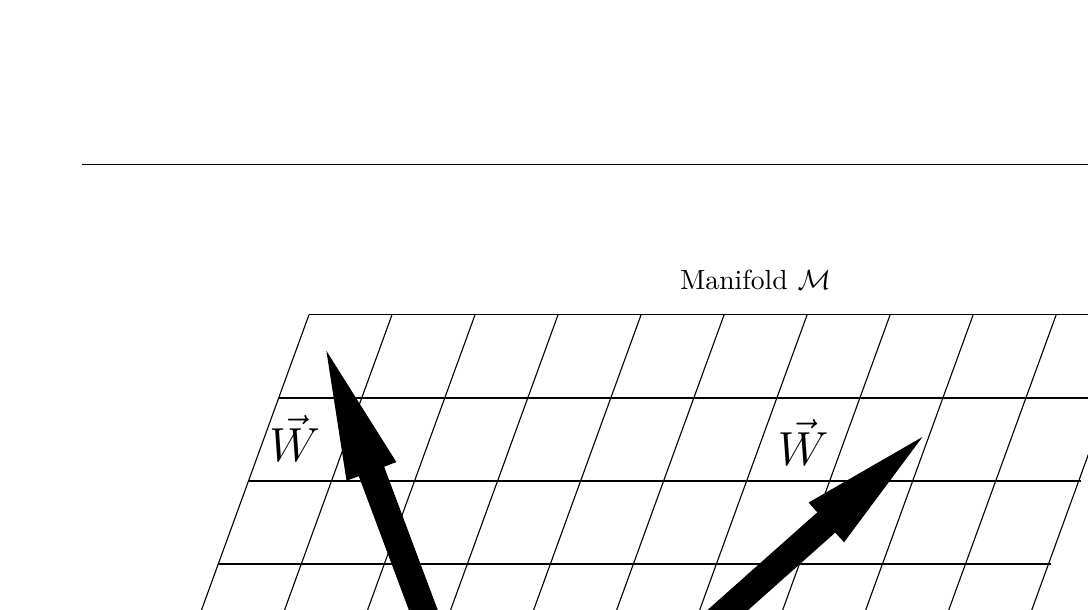
\begin{tikzpicture}[x=0.75pt,y=0.75pt,yscale=-1,xscale=1]
    %uncomment if require: \path (0,300); %set diagram left start at 0, and has height of 300
    
    %Shape: Grid [id:dp5752956801438607] 
    \draw  [draw opacity=0] (171.86,43.69) -- (572.86,43.69) -- (485.14,284.69) -- (84.14,284.69) -- cycle ; \draw  [color={rgb, 255:red, 0; green, 0; blue, 0 }  ,draw opacity=1 ] (171.86,43.69) -- (84.14,284.69)(211.86,43.69) -- (124.14,284.69)(251.86,43.69) -- (164.14,284.69)(291.86,43.69) -- (204.14,284.69)(331.86,43.69) -- (244.14,284.69)(371.86,43.69) -- (284.14,284.69)(411.86,43.69) -- (324.14,284.69)(451.86,43.69) -- (364.14,284.69)(491.86,43.69) -- (404.14,284.69)(531.86,43.69) -- (444.14,284.69)(571.86,43.69) -- (484.14,284.69) ; \draw  [color={rgb, 255:red, 0; green, 0; blue, 0 }  ,draw opacity=1 ] (171.86,43.69) -- (572.86,43.69)(157.3,83.69) -- (558.3,83.69)(142.74,123.69) -- (543.74,123.69)(128.18,163.69) -- (529.18,163.69)(113.62,203.69) -- (514.62,203.69)(99.06,243.69) -- (500.06,243.69)(84.51,283.69) -- (485.51,283.69) ; \draw  [color={rgb, 255:red, 0; green, 0; blue, 0 }  ,draw opacity=1 ]  ;
    %Up Arrow [id:dp6404461279959295] 
    \draw  [fill={rgb, 255:red, 0; green, 0; blue, 0 }  ,fill opacity=1 ] (190.19,123.2) -- (180.74,62.25) -- (213.6,114.45) -- (207.75,116.64) -- (239.48,201.5) -- (227.77,205.88) -- (196.04,121.01) -- cycle ;
    %Straight Lines [id:da8814450115460095] 
    \draw [line width=2.25]    (233.62,203.69) -- (343.01,203.98) ;
    \draw [shift={(347.01,204)}, rotate = 180.16] [color={rgb, 255:red, 0; green, 0; blue, 0 }  ][line width=2.25]    (17.49,-5.26) .. controls (11.12,-2.23) and (5.29,-0.48) .. (0,0) .. controls (5.29,0.48) and (11.12,2.23) .. (17.49,5.26)   ;
    %Up Arrow [id:dp06995273084643272] 
    \draw  [fill={rgb, 255:red, 0; green, 0; blue, 0 }  ,fill opacity=1 ] (413.03,134.15) -- (466.47,103.36) -- (429.64,152.83) -- (425.48,148.16) -- (357.78,208.36) -- (349.47,199.02) -- (417.18,138.82) -- cycle ;
    % Text Node
    \draw (91,199) node  [font=\LARGE] [align=left] {$\displaystyle x_{1}$};
    % Text Node
    \draw (387,27) node   [align=left] {Manifold\textit{ }$\displaystyle \mathcal{M}$};
    % Text Node
    \draw (165,103) node  [font=\LARGE,color={rgb, 255:red, 0; green, 0; blue, 0 }  ,opacity=1 ] [align=left] {$\displaystyle \vec{W}$};
    % Text Node
    \draw (410,105) node  [font=\LARGE,color={rgb, 255:red, 0; green, 0; blue, 0 }  ,opacity=1 ] [align=left] {$\displaystyle \vec{W}$};
    \end{tikzpicture}

    \caption{The Lie derivative gives us information on how the vector $\vec{W}$ changes as it moves along the coordinate $x_1$.}
    \label{fig:ManifoldGrid}
    \end{figure}
    We are interested in only one coordinate, so we will work with the partial derivative along that coordinate as a vector,
    \begin{align}
    \vec{\partial_1} = \vec{\left( \frac{\partial}{\partial x_1} \right)}.
    \end{align}
    Since it is a vector, we can also bring it down into components:
    \begin{align}
    \vec{V} = \vec{\partial_1} = V^{\mu} \vec{\partial_{\mu}},
    \end{align}
    \begin{align}
        V^{\mu} &= \begin{pmatrix}
               0 \\
               1 \\
               0 \\
               0
             \end{pmatrix} =  \delta_1^{\mu}.
    \end{align}
    The components of the Lie derivative acting on $\vec{W}$ in the $x_1$ direction are given by
    \begin{align}
        \left(\mathcal{L}_{\vec{\partial_1}} \vec{W} \right)^{\mu} = \delta_1^{\alpha} \partial_{\alpha} W^{\mu} - W^{\alpha} \partial_{\alpha} \delta_1^{\mu} = \partial_1 W^{\mu},
    \end{align}
    which is just the partial derivative in the $x_1$ direction. This can be used as a way to determine if a vector field does not change in a certain direction. For instance, let $W^{\mu} = W^{\mu}(x^0,x^2,x^3)$, then $\left( \mathcal{L}_{\vec{\partial_1}} \vec{W} \right)^{\mu} = 0$. 
    %
    As an example, let's imagine that we take the Lie derivative of the metric in the $\phi$ direction of the two-dimensional sphere $S^2$, as in Fig. \ref{fig:S2}. It's not hard to see that we can spin the 2-sphere in the $\phi$ direction and its shape would remain the same. Acting with a Lie derivative on the metric along $\phi$ would give zero, so we can say that it is a symmetry of our spacetime. In this case, we know that $g_{\mu \nu}$ will be a function of the polar angle $\theta$ only, according to our choice of coordinates.
    
    \begin{figure}[h]
        \centering
        \tikzset{every picture/.style={line width=0.75pt}} %set default line width to 0.75pt        
        
        \begin{tikzpicture}[x=0.75pt,y=0.75pt,yscale=-1,xscale=1]
        %uncomment if require: \path (0,300); %set diagram left start at 0, and has height of 300
        
        %Shape: Circle [id:dp6180128382661292] 
        \draw   (167,154.5) .. controls (167,90.71) and (218.71,39) .. (282.5,39) .. controls (346.29,39) and (398,90.71) .. (398,154.5) .. controls (398,218.29) and (346.29,270) .. (282.5,270) .. controls (218.71,270) and (167,218.29) .. (167,154.5) -- cycle ;
        %Shape: Ellipse [id:dp42044654160980244] 
        \draw  [dash pattern={on 4.5pt off 4.5pt}] (167,154.5) .. controls (167,143.45) and (218.71,134.5) .. (282.5,134.5) .. controls (346.29,134.5) and (398,143.45) .. (398,154.5) .. controls (398,165.55) and (346.29,174.5) .. (282.5,174.5) .. controls (218.71,174.5) and (167,165.55) .. (167,154.5) -- cycle ;
        %Shape: Arc [id:dp8891000319294102] 
        \draw  [draw opacity=0] (387.25,107.83) .. controls (375.23,117.33) and (333.96,124.97) .. (284.74,125.95) .. controls (225.94,127.12) and (178.08,118.33) .. (177.84,106.33) .. controls (177.83,105.8) and (177.92,105.26) .. (178.09,104.73) -- (284.31,104.21) -- cycle ; \draw   (387.25,107.83) .. controls (375.23,117.33) and (333.96,124.97) .. (284.74,125.95) .. controls (225.94,127.12) and (178.08,118.33) .. (177.84,106.33) .. controls (177.83,105.8) and (177.92,105.26) .. (178.09,104.73) ;
        %Shape: Arc [id:dp9250724757620967] 
        \draw  [draw opacity=0] (386.25,202.83) .. controls (374.23,212.33) and (332.96,219.97) .. (283.74,220.95) .. controls (224.94,222.12) and (177.08,213.33) .. (176.84,201.33) .. controls (176.83,200.8) and (176.92,200.26) .. (177.09,199.73) -- (283.31,199.21) -- cycle ; \draw   (386.25,202.83) .. controls (374.23,212.33) and (332.96,219.97) .. (283.74,220.95) .. controls (224.94,222.12) and (177.08,213.33) .. (176.84,201.33) .. controls (176.83,200.8) and (176.92,200.26) .. (177.09,199.73) ;
        \draw   (262,169) -- (292,174.5) -- (262,180) ;
        \draw   (264,120) -- (294,126) -- (264,132) ;
        \draw   (264,215) -- (294,221) -- (264,227) ;
        
        % Text Node
        \draw (157,61) node  [font=\huge] [align=left] {$\displaystyle S^{2}$};
        % Text Node
        \draw (303,195) node  [font=\Large] [align=left] {$\displaystyle \overrightarrow{\partial _{\phi }}$};
        
        
        \end{tikzpicture}

        \caption{If the Lie derivative of the metric along the $\phi$ direction on the 2-sphere is zero, we know that $g_{\mu \nu}=g_{\mu \nu} (\theta).$}
        \label{fig:S2}
    \end{figure}
    
    With this analysis, we can draw two important conclusions:
    \begin{enumerate}
        \item If $\mathcal{L}_{\vec{K}} g = 0$, then there is a symmetry of the spacetime.
        \item If $g$ doesn't depend on a particular coordinate (say, $x^1$) then $\vec{K} = \vec{\partial_1}$ is a ``Killing vector (field)'' and there is a symmetry.
    \end{enumerate}
    
    \section{Covariant derivative}
    
    Once defined, the covariant derivative will give us a notion of how to take a directional derivative in spacetime as well as what we really mean by a geodesic. While we won't have the full story about how things behave in curved spacetime, we will know a lot about how objects move in curved spacetime.
    
    Our approach will be to build a derivative that will satisfy certain conditions. We want to work with a derivative that, when acting on a given tensor field, it will produce a new tensor, i.e. $\nabla: (k,l) \rightarrow (k,l+1)$. The rank of the new tensor can be guessed by remembering that the partial derivative acting on a scalar function, which is a rank-(0,0) tensor, produces a rank-(0,1) tensor.
    
    Now, we want this new mathematical object to behave both as a tensor as well as a derivative. We will ask six things to be satisfied by it in order to define it in an appropriate, unique way. These properties are:
    \begin{enumerate}
        \item Linearity: for two coefficients $a$, $b$ and two tensor fields $T$, $S$ we want 
        \begin{align}
            \nabla(a T + b S) = a \nabla T + b \nabla S
        \end{align}
        
        \item Leibniz rule: 
        \begin{align}
            \nabla (T \otimes S) = (\nabla T) \otimes S + T \otimes (\nabla S)
        \end{align}
        Let's see how this would work for a vector field $\vec{W}$:
        \begin{align}
            \nabla \vec{W} = \left(\nabla_{\mu} W^{\nu} \right) \undertilde{d} x^{\mu} \otimes \vec{\partial_{\nu}}.
        \end{align}
        We guess that the components will look like this
        \begin{align}
            \nabla_{\mu} W^{\nu} = \partial_{\mu} W^{\nu} + \left( \Gamma_{\mu} \right)^{\nu}_{\alpha} W^{\alpha},
        \end{align}
        where we introduced the four 4x4 matrices $\left( \Gamma_{\mu} \right)^{\nu}_{\alpha}$ in order to have a linear operator. We will insist that the connection coefficients $\Gamma_{\mu \nu}^{\rho}$ in just the right way such that
        \begin{align}
            \nabla_{\mu'} W^{\mu'} = \frac{\partial x^{\mu}}{\partial x^{\mu'}} \frac{\partial x^{\nu'}}{\partial x^{\nu}} \nabla_{\mu} W^{\nu},
        \end{align}
        which also means that the connection coefficients do not transform as tensors since the partial derivative of a general tensor does not transform as such. The transformation of the coefficients is given by
        \begin{align}
            \Gamma_{\mu' \lambda'}^{\nu'} = \frac{\partial x^{\mu}}{\partial x^{\mu'}} \frac{\partial x^{\lambda}}{\partial x^{\lambda'}} \frac{\partial x^{\nu'}}{\partial x^{\nu}} \Gamma_{\mu \lambda}^{\nu} - \frac{\partial x^{\mu}}{\partial x^{\mu'}} \frac{\partial x^{\lambda}}{\partial x^{\lambda'}} \frac{\partial^2 x^{\nu'}}{\partial x^{\mu} \partial x^{\lambda}}.
        \end{align}
        
        \item We want the covariant derivative to reduce to a partial derivative when it acts on a scalar function:
        \begin{align}
            \nabla_{\mu} f = \partial_{\mu} f.
        \end{align}
        
        \item $\nabla$ respects contractions, i.e.
        \begin{align}
            \nabla_{\mu} \left(T^{\alpha}_{\ \nu \alpha} \right) = \left(\nabla T \right)_{\mu}^{\ \alpha}_{\nu \alpha}
        \end{align}
        
        At this point, we can extend this derivative to all objects. The natural question to ask is, how does the covariant derivative act on 1-forms?
        \begin{align}
            \nabla_{\mu} \omega_{\nu} = \partial_{\mu} \omega_{\nu} + \Tilde{\Gamma}^{\alpha}_{\mu \nu} \omega_{\alpha}.
        \end{align}
        The index order is not important as the connection coefficients are not really tensors. However, if necessary, the following convention can be used: $\Gamma^{\rho}_{\mu \nu} = \Gamma^{\rho}_{\ \mu \nu}$.
        
        Let's figure out what the $\Tilde{\Gamma}$ are by taking the derivative of the following contraction:
        \begin{align}
            \nabla_{\mu} (V^{\alpha} \omega_{
            \alpha}) &= \partial_{\mu} (V^{\alpha} \omega_{\alpha}) \nonumber \\
            &= (\nabla_{\mu}V^{\alpha}) \omega_{\alpha} + V^{\alpha} (\nabla_{\mu} \omega_\alpha) \nonumber\\
            &= \left(\partial_{\mu} V^{\alpha} + \Gamma_{\mu \beta}^{\alpha} V^{\beta} \right) \omega_{\alpha} + \left(\partial_{\mu} \omega_{\alpha} + \Tilde{\Gamma}_{\mu \alpha}^{\beta} \omega_{\beta} \right) V^{\alpha}\nonumber
            \end{align}
            \begin{align}
            &\Rightarrow 0 =V^{\alpha} \left( \Gamma_{\mu \alpha}^{\beta} + \Tilde{\Gamma}_{\mu \alpha}^{\beta} \right) \omega_{\beta}\nonumber\\
            &\Rightarrow \Tilde{\Gamma}_{\mu \nu}^{\rho} = - \Gamma_{\mu \nu}^{\rho}.
        \end{align}
        
        So now we can determine how $\nabla$ acts on any tensor. For instance, let $T^{\mu}_{\ \nu}$ be a (1,1)-tensor:
        \begin{align}
            \nabla_{\mu} T^{\nu}_{\ \rho} = \partial_{\mu} T^{\nu}_{\ \rho} + \Gamma^{\nu}_{\mu \alpha} T^{\alpha}_{\ \rho} - \Gamma^{\alpha}_{\mu \rho} T^{\nu}_{\ \alpha}.
        \end{align}
        
        With what we know so far about the connection coefficients following the rules we have stated, we can actually build a tensor with them. Consider two different sets of coefficients $\Gamma$, $\hat{\Gamma}$ and take the difference
        \begin{align*}
            \nabla_{\mu} V^{\nu} - \hat{\nabla}_{\mu} V^{\nu} &= \partial_{\mu} V^{\nu} + \Gamma_{\mu \alpha}^{\nu} V^{\alpha} - \partial_{\mu} V^{\nu} - \hat{\Gamma}_{\mu \alpha}^{\nu} V^{\alpha} \\
            &= \left(\Gamma_{\mu \alpha}^{\nu}-\hat{\Gamma}_{\mu \alpha}^{\nu} \right).
        \end{align*}
        Since $\nabla_{\mu} V^{\nu} - \hat{\nabla}_{\mu} V^{\nu}$ is a tensor, the object
        \begin{align}
            S_{\mu \alpha}^{\nu} = \Gamma_{\mu \alpha}^{\nu}-\hat{\Gamma}_{\mu \alpha}^{\nu}
        \end{align}
        must be a tensor.
        
        Before we state the next property, let's consider the following object associated to any given connection:
        \begin{align}
            T^{\rho}_{\ \mu \nu} = \Gamma^{\rho}_{\ \mu \nu} - \Gamma^{\rho}_{\ \nu \mu} = 2 \Gamma^{\rho}_{\ [\mu \nu]}.
        \end{align}
        This object is known as the \textbf{torsion tensor}, and clearly it is antisymmetric in its lower indices. A connection that is symmetric in its lower indices is known as ``torsion-free''. With this in mind, we can ask our connection coefficients to be
        \item Torsionless or torsion-free:
        \begin{align}
            T^{\rho}_{\ \mu \nu} = 0.
        \end{align}
        
        \item Finally, we want metric compatibility
        \begin{align}
            \nabla_{\mu} g_{\nu \rho} = 0.
        \end{align}
        This makes the connection unique. There are several consequences to this, such as
        \begin{align*}
            \nabla_{\mu} \left(V^{\alpha} W_{\alpha} \right) &= \nabla_{\mu} \left(V^{\alpha} W^{\beta} g_{\alpha \beta} \right)\\
            &= g_{\alpha \beta} \nabla_{\mu} \left(V^{\alpha} W^{\beta} \right)\\
            &= \nabla_{\mu} \left(V_{\alpha} W_{\beta} g^{\alpha \beta} \right),
        \end{align*}
        \begin{align*}
            \nabla_{\mu} g^{\rho \sigma} &= 0,\\
            \nabla_{\mu} g &= 0,\\
            \nabla_{\alpha} \epsilon_{\mu \nu \rho \sigma} &= 0,
        \end{align*}
        where $g$ is the trace of the metric tensor and $\epsilon_{\mu \nu \rho \sigma}$ is the Levi-Civita tensor.
    \end{enumerate}
    
%%%%%%%%%%%%%%%%%%%%%%%%%%%%%%%%%%%%%%%%%%
\end{document}